\documentclass[tikz,border=6pt]{standalone}
% =============================================================================
%  PREAMBULE COMMUN DES SCHEMAS DU SUPPORT DE SOUTENANCE (ENSAE, octobre 2026)
%
%  Les schemas sont des VISUELS DE DIAPOSITIVE, pas des figures de donnees : ils
%  prennent donc la palette du gabarit de presentation Nexialog, recopiee de
%  build_soutenance_ppt.py, et jamais celle de style_nexialog.py, qui reste la
%  source unique des couleurs des figures du memoire.
%
%  AUCUN NOMBRE DE RESULTAT N'Y FIGURE. Un nombre dessine dans une image echappe
%  au controle du support, qui verifie chaque nombre de texte contre le rapport.
%  Les schemas portent des symboles et des equations, recopiees du rapport.
%
%  Polices : Segoe UI pour le texte, comme le corps du gabarit ; Latin Modern Math
%  pour les formules, celle du rapport. Chaque schema se dessine A SA TAILLE FINALE
%  sur la diapositive, si bien qu'un corps de 14 pt ici vaut 14 pt a l'ecran.
% =============================================================================
\usepackage{fontspec}
\usepackage{unicode-math}
\setmainfont{Segoe UI}
\setsansfont{Segoe UI}
\setmathfont{latinmodern-math.otf}
\usetikzlibrary{positioning,arrows.meta,calc,fit,backgrounds,shapes.geometric,decorations.pathreplacing}

\definecolor{ardoise}{HTML}{223E55}   % titres et aplats du gabarit
\definecolor{profond}{HTML}{192E3F}
\definecolor{acier}{HTML}{435B6E}
\definecolor{encre}{HTML}{122738}     % texte courant
\definecolor{gris}{HTML}{595959}      % texte secondaire
\definecolor{accent}{HTML}{B10031}    % rouge de marque
\definecolor{clair}{HTML}{F2F2F2}
\definecolor{filet}{HTML}{D9D9D9}

\newcommand{\corps}{\fontsize{14}{17}\selectfont}
\newcommand{\petit}{\fontsize{12}{14.5}\selectfont}
\newcommand{\grand}{\fontsize{16}{19}\selectfont}
\tikzset{
  >={Stealth[length=7pt,width=6pt]},
  bloc/.style={draw=ardoise, line width=0.9pt, fill=white, rounded corners=3pt,
               inner sep=6pt, align=center, text=encre, font=\corps},
  bloc plein/.style={fill=ardoise, draw=ardoise, rounded corners=3pt, inner sep=6pt,
               align=center, text=white, font=\corps\bfseries},
  bloc accent/.style={fill=accent, draw=accent, rounded corners=3pt, inner sep=6pt,
               align=center, text=white, font=\corps\bfseries},
  fleche/.style={->, line width=1.3pt, draw=acier},
  fleche accent/.style={->, line width=1.6pt, draw=accent},
  legende/.style={font=\petit, text=gris, align=center},
}

% Illustration qualitative de l'inversion de deux probabilites de transmission.
% Aucun nombre de calibration ; les resultats de capital portent sur les cinq piliers.
\begin{document}
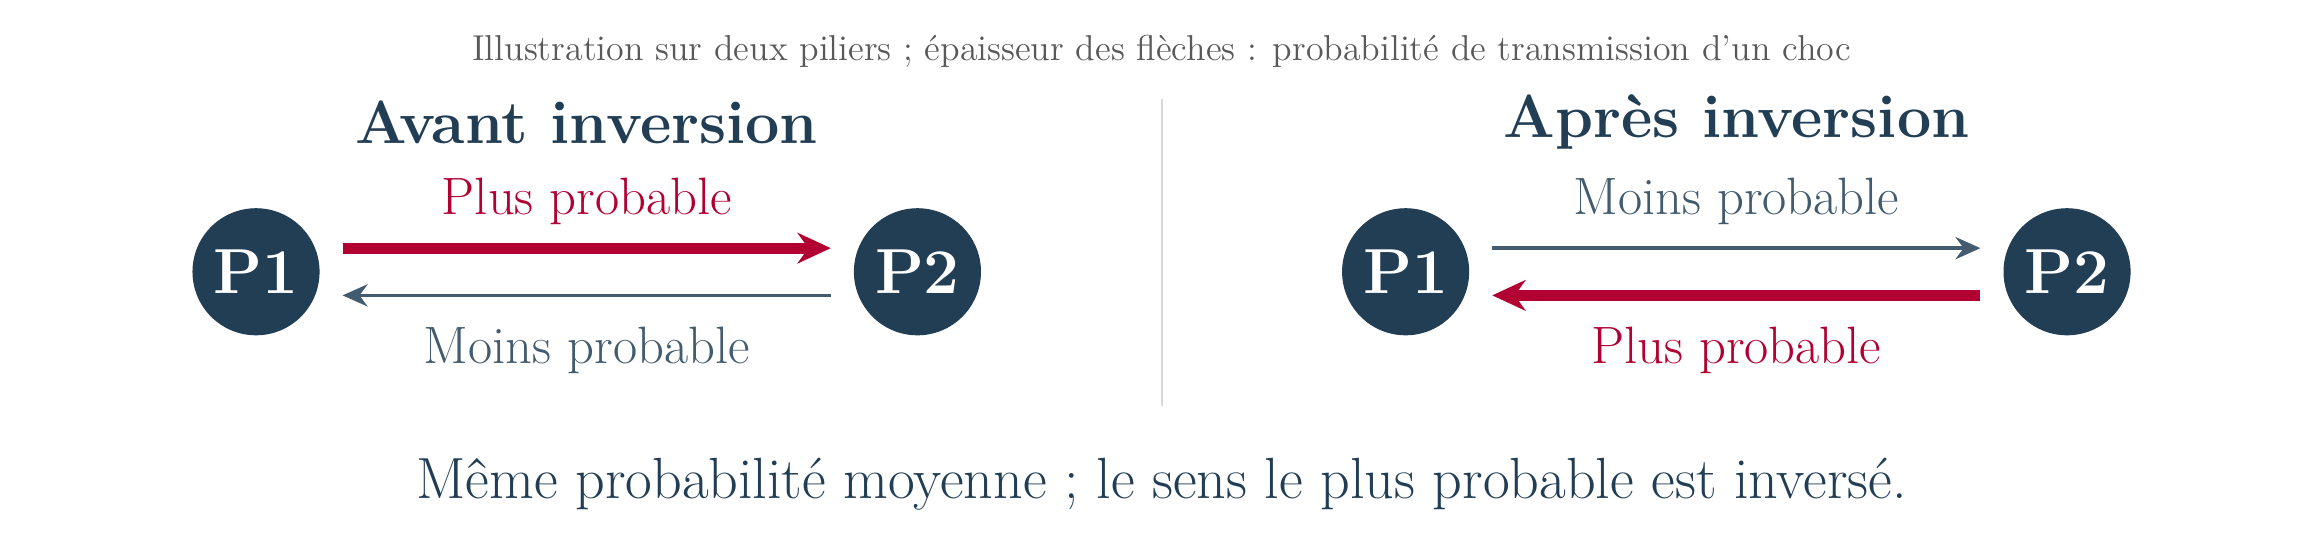
\begin{tikzpicture}[
  pilier/.style={circle,fill=ardoise,draw=ardoise,text=white,minimum size=1.6cm,
    inner sep=0pt,font=\fontsize{23}{26}\selectfont\bfseries},
  titre/.style={font=\fontsize{22}{25}\selectfont\bfseries,text=ardoise,align=center},
  legende/.style={font=\fontsize{19}{22}\selectfont,align=center},
  fort/.style={-{Stealth[length=12pt,width=11pt]},draw=accent,line width=4pt},
  faible/.style={-{Stealth[length=9pt,width=8pt]},draw=acier,line width=1.3pt}]
  \useasboundingbox (0,0) rectangle (28.8,6.4);
  \node[font=\fontsize{13}{16}\selectfont,text=gris] at (14.4,6.1)
    {Illustration sur deux piliers ; épaisseur des flèches : probabilité de transmission d'un choc};
  \node[titre] at (7.1,5.2) {Avant inversion};
  \node[titre] at (21.7,5.2) {Après inversion};
  \draw[filet,line width=.7pt] (14.4,1.6)--(14.4,5.5);
  \node[pilier] (a1) at (2.9,3.3) {P1};
  \node[pilier] (a2) at (11.3,3.3) {P2};
  \draw[fort] (4.0,3.6)--(10.2,3.6);
  \draw[faible] (10.2,3.0)--(4.0,3.0);
  \node[legende,text=accent] at (7.1,4.2) {Plus probable};
  \node[legende,text=acier] at (7.1,2.3) {Moins probable};
  \node[pilier] (b1) at (17.5,3.3) {P1};
  \node[pilier] (b2) at (25.9,3.3) {P2};
  \draw[faible] (18.6,3.6)--(24.8,3.6);
  \draw[fort] (24.8,3.0)--(18.6,3.0);
  \node[legende,text=acier] at (21.7,4.2) {Moins probable};
  \node[legende,text=accent] at (21.7,2.3) {Plus probable};
  \node[font=\fontsize{21}{24}\selectfont,text=ardoise,align=center] at (14.4,.6)
    {Même probabilité moyenne ; le sens le plus probable est inversé.};
\end{tikzpicture}
\end{document}
